% -*- root: ../EstadisticaII.tex -*-
\chapter{Clasificación}


Disponemos de una muestra de $k$ variables medidas en $n$ unidades u objetos que pertenecen a dos grupos o poblaciones \textit{(training data)}.

Cada observación $i=1,\ldots,n$ consiste en un vector $(x'_i,y_i)'$, donde $x_i\in\mathbb{R}^k$ son las $k$ variables e    $y\in\{0,1\}$ indica el grupo al que pertenece la unidad en la que se han obtenido. 

\textbf{Objetivo:} Asignar una nueva unidad con valores $x$ (e $y$ desconocida) a uno de los dos grupos (\textbf{obtener una regla de clasificación}).


Este problema tiene diferentes nombres en la literatura en inglés: ``supervised classification", ``statistical learning", ``discrimination", ``machine learning", ``pattern recognition", etc.

Vamos a ver un ejemplo, para entender mejor el tema

\begin{example}
En un estudio de factores de riesgo en enfermedades coronarias, se dispone de datos de 462 personas (de las que 160 habían sufrido infartos y 302 eran controles). Para cada una de ellas se midieron las siguientes variables:


\begin{center}
\label{example:infartos}
{\scriptsize

\begin{tabular}{|c|l|}
\hline Nombre variable & Descripci\'{o}n  \\
\hline {\tt sbp} & Tensión sanguínea sistólica \\
{\tt tobacco} & Consumo de tabaco\\
{\tt ldl} & Colesterol\\
{\tt adiposity} & Medida de adiposidad\\
{\tt typea} & Comportamiento ``tipo A"\\
{\tt obesity} & Medida de la obesidad\\
{\tt alcohol} & Consumo de alcohol\\
{\tt age} & Edad \\
 \hline
 \end{tabular}

 }
\end{center}

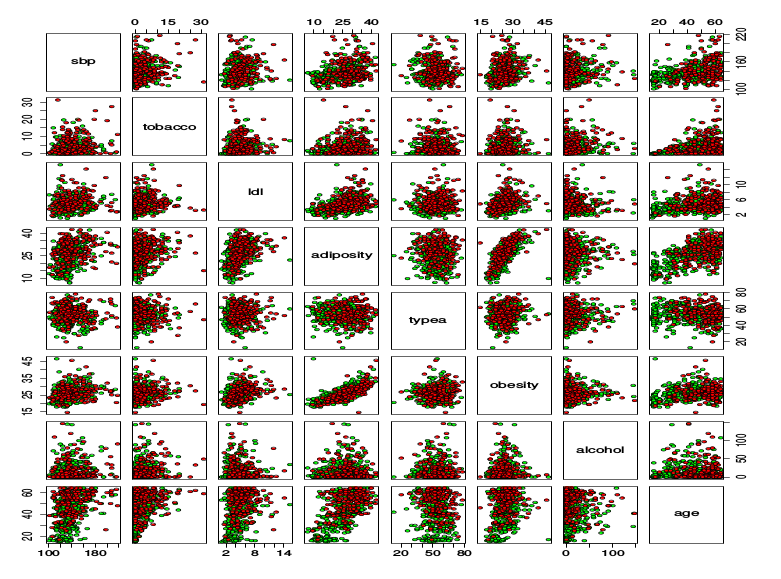
\includegraphics[width=13 cm]{img/pairs-heart.png}


Ahora nos gustaría poder predecir si un nuevo individuo va a tener un infarto o no en función de su consumo de tabaco, colesterol, ...
\end{example}


\section{Regla de Mahalanobis}

La idea es asignar el nuevo individuo al grupo cuyo centro es más cercano (cercano en el sentido de la distancia de Mahalanobis).


\begin{defn}[Regla\IS de Mahalanobis]
Para $i=0,1$ denotamos $P_i$  a la distribución condicionada  $X|Y=i$. Suponemos que $P_i$ es una distribución con vector de medias $\mu_i$ y matriz de covarianzas $\Sigma_i$.


\textbf{Regla de Mahalanobis:} Clasificar $x$ en el grupo 1 (i.e. $Y=1$) si y solo si
\[
(x-\mu_0)'\Sigma_0^{-1}(x-\mu_0) >  (x-\mu_1)'\Sigma_1^{-1}(x-\mu_1).
\]
\end{defn}
En la práctica se usan los vectores de medias y las matrices de covarianzas muestrales, ya que no disponemos de los reales.

La frontera de clasificación sería cuando 
\[
(x-\mu_0)'\Sigma_0^{-1}(x-\mu_0) =  (x-\mu_1)'\Sigma_1^{-1}(x-\mu_1).
\]

Esta frontera será una curva cuadrática (por ser una igualdad entre formas cuadráticas). 

\begin{example}


\centerline{$\mu_0=(1,0)^\prime$, $\mu_1=
(5,0)^\prime$, $\Sigma_1=\left[
  \begin{array}{cc}
    1 & 0 \\
    0 & 1 \
  \end{array} \right]$,
$\Sigma_2=\left[
  \begin{array}{cc}
    5 & 0 \\
    0 & 5 \
  \end{array} \right]$.}

\begin{center}
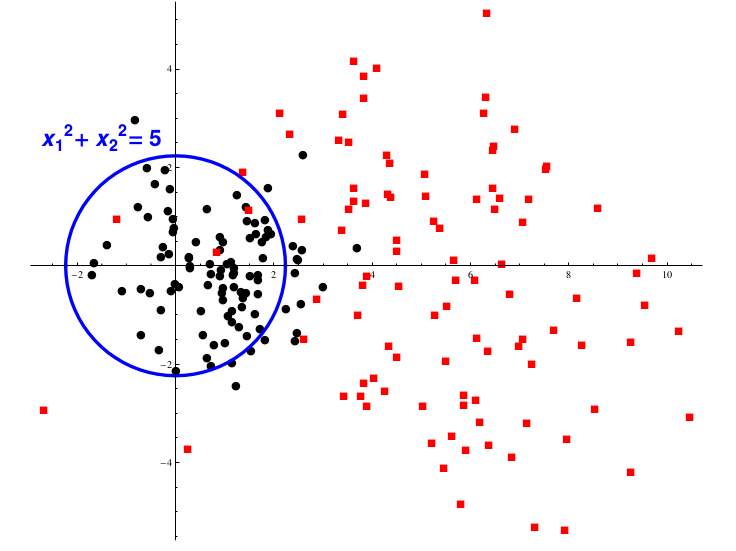
\includegraphics[width=13 cm]{img/ReglaMahalanobis.png}
\end{center}

\end{example}

\section{Regla de Fisher}

Vamos a suponer $Σ_1 = Σ_0$, que es cuando mejor funciona esta regla. Vamos a suponer que tenemos estos datos:

\begin{center}
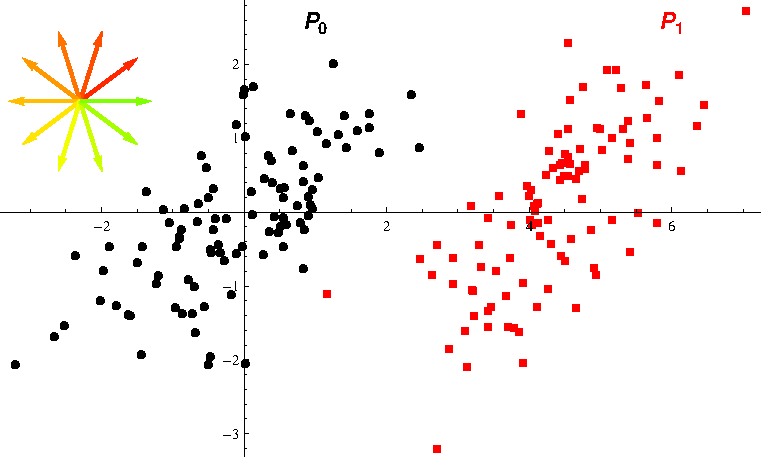
\includegraphics[width=13 cm]{pdf/tema4/_Fisher}
\end{center}


Y la idea intuitiva es construir una recta sobre la que proyectar, para construir 2 histogramas. Si nos dan un nuevo dato, lo clasificaremos en el histograma al que sea más probable que pertenezca.

\begin{center}
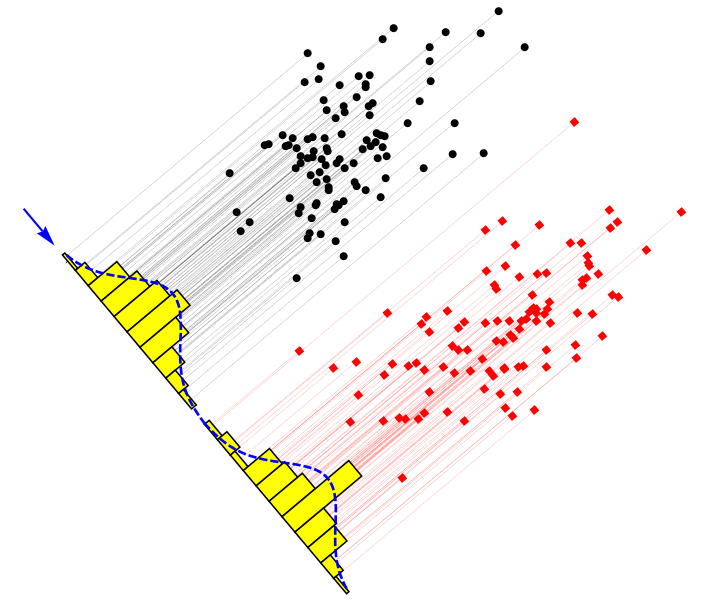
\includegraphics[width=13 cm]{img/ReglaFisherIntuitiva.png}
\end{center}


\paragraph{¿Cómo construir esta recta?} Tenemos que tener en cuenta 2 cosas:


\begin{itemize}
  \item Una buena direcci\'{o}n debe separar bien los centros de los grupos. La distancia entre las medias $(a'\mu_0-a'\mu_1)^2 = a'Ba$, donde $B=(\mu_0-\mu_1)(\mu_0-\mu_1)'$, debe ser grande.

\centerline{{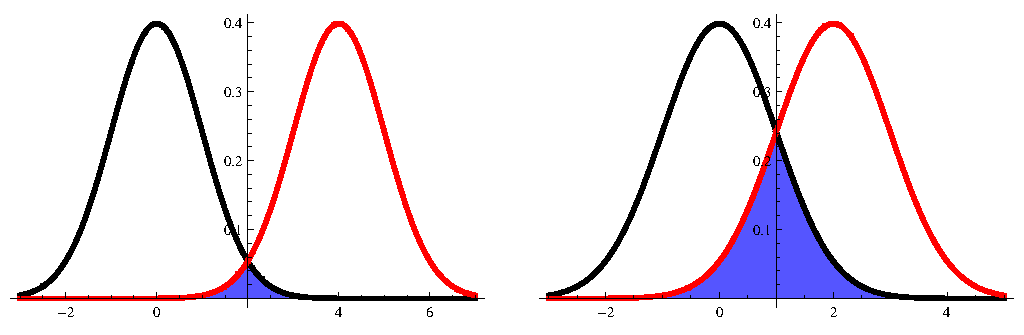
\includegraphics[width=13 cm]{pdf/tema4/_Fisher-normales-1}}}

  \item La varianza de las proyecciones dentro de los grupos ($a'\Sigma a$) debe ser lo menor
  posible.

\centerline{{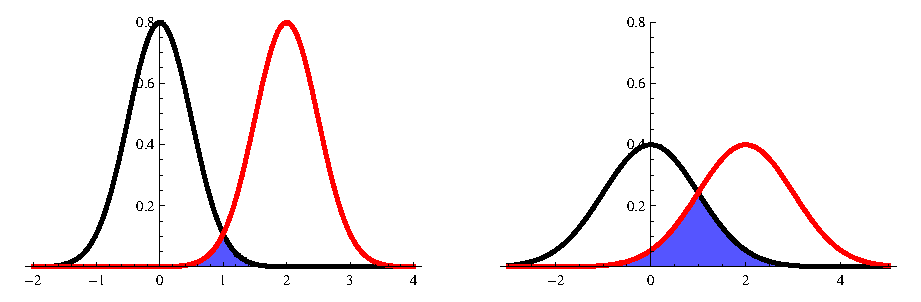
\includegraphics[width=13 cm]{pdf/tema4/_Fisher-normales-2}}}

\end{itemize}


La idea de Fisher fue maximizar el ratio de la separación de los centros entre las varianzas, es decir, maximizar el \concept{Cociente\IS de Rayleigh}

\[
f(a) = \frac{a'Ba}{a'\Sigma a} 
\]

para cualquier dirección $a∈ℝ^n$.

\obs Este problema tiene infinitas soluciones, ya que $f(a) = f(λa) ∀λ∈ℝ$. Para solucionar esto, imponemos la normalización tal que $a'Σa = 1$ (aunque no sea la única).

Vamos a calcular el máximo de esta función\footnote{Utilizamos $\grad a'Σa = 2aΣ$. La derivada de una forma cuadrática que es algo que ya deberíamos haber sabido de otras asignaturas del grado.}

\[
\grad f(a) = \frac{2Ba(a'Σa) - 2Σa(a'Ba)}{(a'Σa)^2} \to \grad f(ω) = 0 \dimplies Bω(ω'Σω) = Σω(ω'Bω)
\]

Si llegamos a encontrar ese $ω$, tendrá estas 2 propiedades
\begin{itemize}
	\item $Bω = (µ_0-µ_1)\underbrace{(µ_0 - µ_1)'ω}_{α}$ siendo $α$ un escalar. Esto quiere decir que $Bω = (µ_0-µ_1)α$, esto es: $Bω$ es proporcional a $µ_0 - µ_1$. 
	\item $Σω$ es proporcional a $Σ^{-1}(µ_0 - µ_1)$
\end{itemize}

\begin{defn}[Regla\IS de Fisher] Clasificar $x$ en el grupo 1 (i.e. $Y=1$) si y solo si
\[
ω'\left(x-\frac{\mu_0 + \mu_1}{2}\right)>0
\]
donde $ω=\Sigma^{-1}(\mu_1-\mu_0).$

En caso de tener $ω'\left(x-\frac{\mu_0 + \mu_1}{2}\right)<0$, clasificaríamos en el grupo 2.
\end{defn}

\obs Esta regla funciona bien cuando $Σ_0 = Σ_1$, es decir, las nubes de puntos tienen la misma forma y orientación. ¿Qué ocurre cuando las matrices de covarianzas son distintas?

\begin{center}
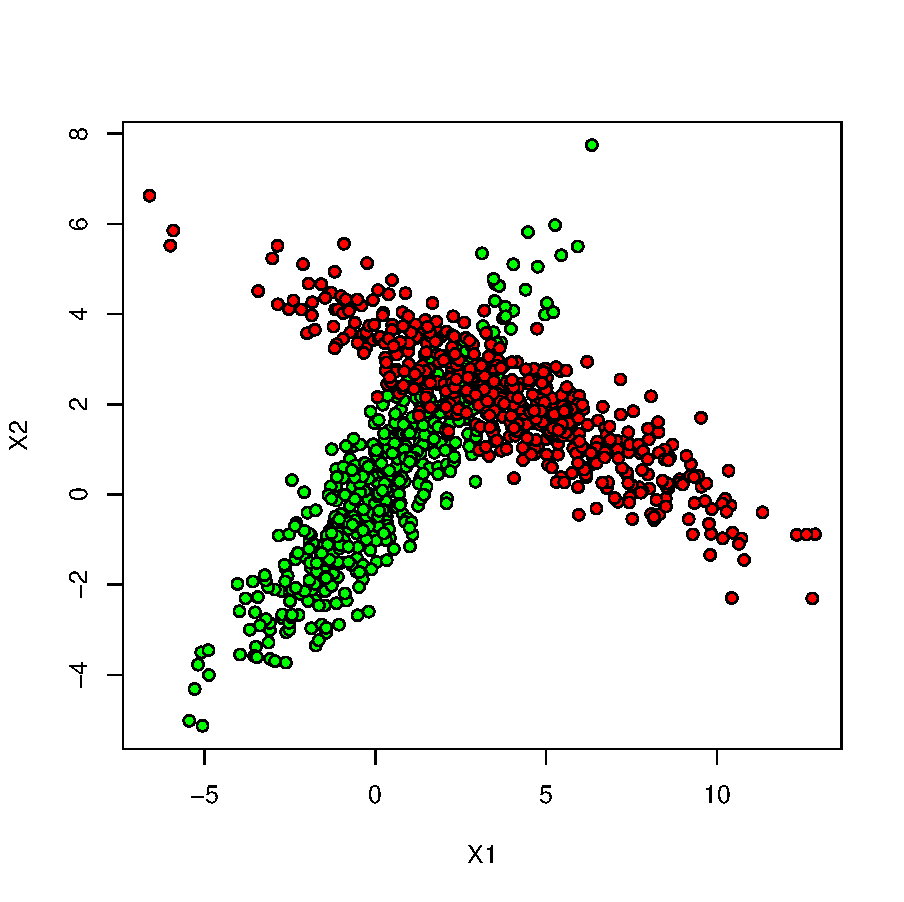
\includegraphics[width=13 cm]{pdf/tema4/_sim-plot}
\end{center}

En la imagen vemos que la regla de Fisher (recta azul) no divide nada bien los datos. Por otro lado, vemos la división por la distancia de Mahalanobis (en rojo) que es mucho más adecuada.

\begin{center}
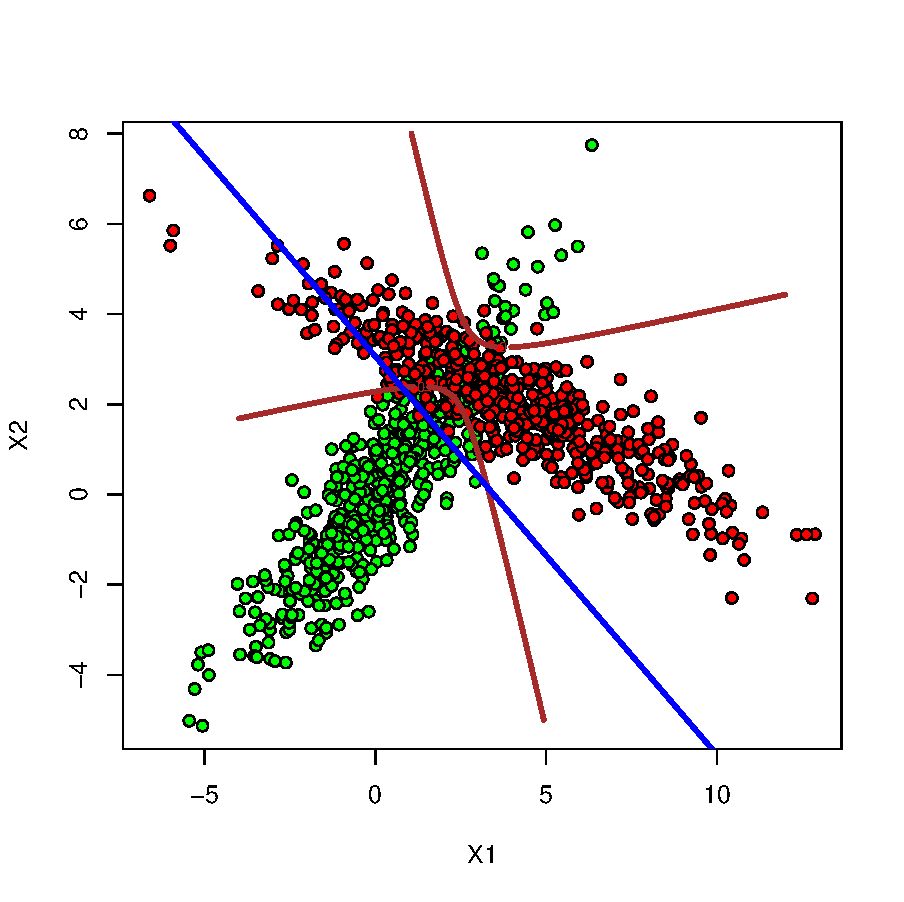
\includegraphics[width=13 cm]{pdf/tema4/_sim-plot-reglas}
\end{center}


\subsection{Validación del modelo}

Acabamos de ver un ejemplo de un caso en el que vemos (a simple vista) que un modelo clasifica mejor que el otro. ¿Porqué sabemos que es mejor? Porque comete menos errores. Vamos a ver en esta sección cómo calcular errores.

\centerline{{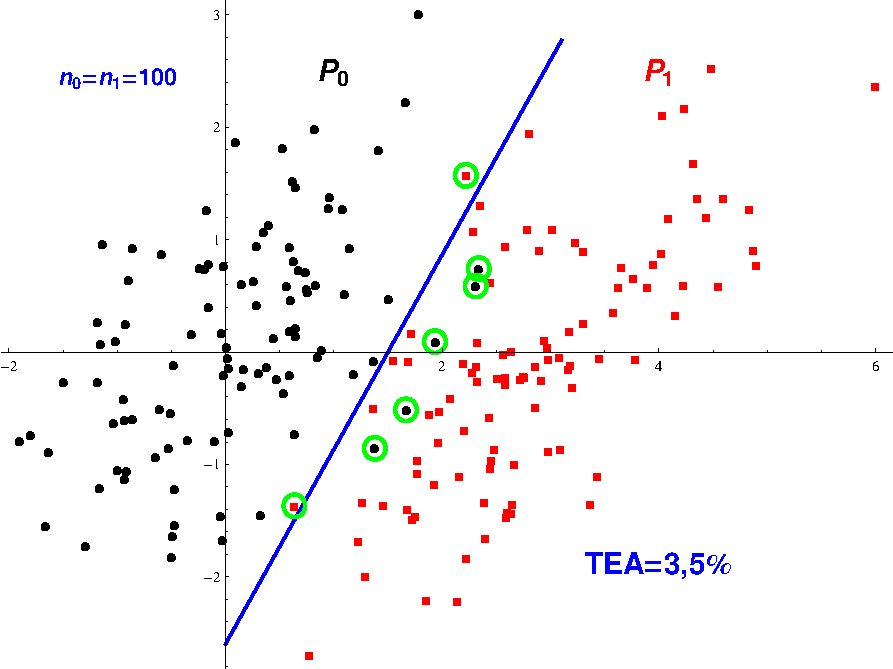
\includegraphics[width=13 cm]{pdf/tema4/_errores-1}}}

\begin{defn}[Tasa de error aparente]
$$\text{TEA}:=\frac{\text{Total de mal clasificados en la muestra}}{n}100\%.$$
\end{defn}

El problema de esta tasa de error es que infraestima la tasa de error. Esto se debe a que estamos utilizando los mismos puntos para construir el modelo y para evaluarlo. 

La solución es la creación de particiones de train y de test. De esta manera utilizamos los datos de train para construir el modelo y el de test para evaluarlo. ¿Y cómo asegurar que la tasa de error no depende de las particiones construidas? No se puede, pero lo que podemos hacer es utilizar la Validación cruzada.

\begin{defn}[Validación\IS cruzada]Omitimos un dato de los n observados y generamos la regla de clasificación con los n − 1 restantes. Clasificamos la observación apartada y repetimos el procedimiento para cada una de las observaciones.
\end{defn}


\section{Regresión logística}

Vamos a recordar el ejemplo de infartos de miocardio y vamos a ver cómo clasifican los modelos de clasificación estudiados hasta ahora.

En rojo vemos utilizando la distancia de Mahalanobis y en azul la regla de Fisher.
\centerline{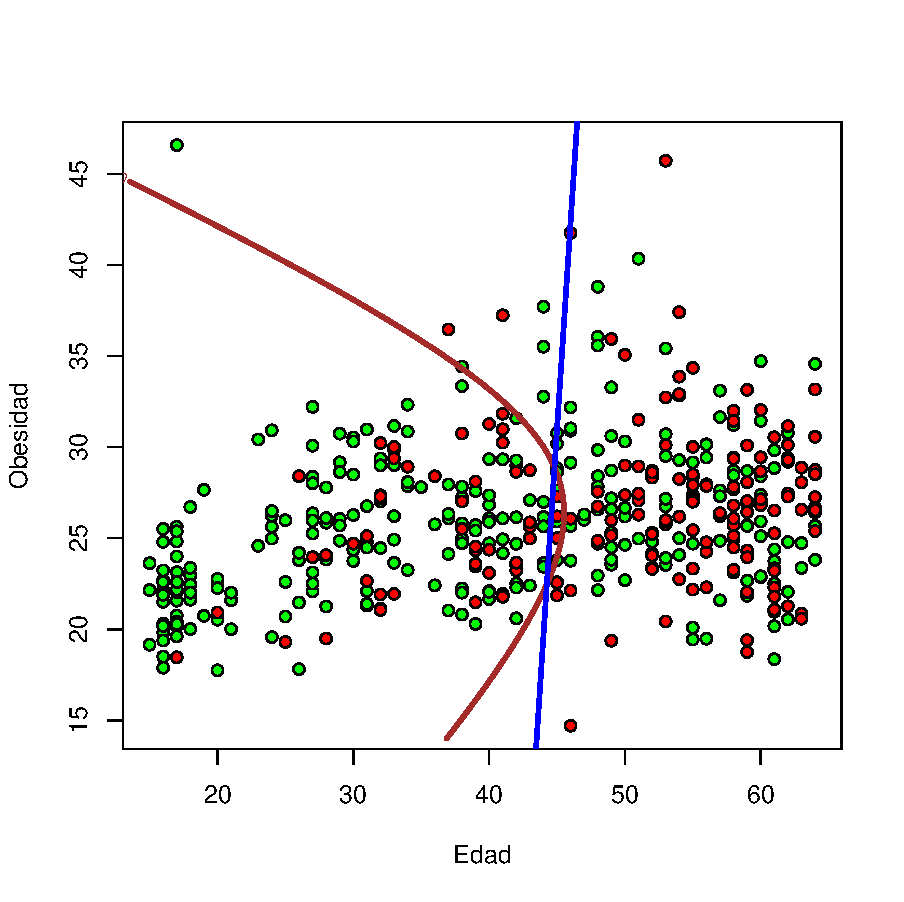
\includegraphics[width=13 cm]{pdf/tema4/_edadobesidad-reglas}}

Vemos que ninguno de los 2 es bueno. Por ello, vamos a ver otro método de clasificación planteando  la clasificación como un problema de regresión múltiple. 

No podemos utilizarlo como tal porque la variable regresora $Y_i$ es binaria y en la regresión múltiple era continua (más concretamente normal). Por ello, hay que buscar una alternativa.


\subsection{Construcción del modelo}
Las variables $Y_1,\ldots,Y_n$ son independientes y tienen distribución de Bernoulli. 

Denotamos $p_i=\mathbb{P}(Y_i=1 \mid x_i)$. La probabilidad de ``éxito'' depende de las variables regresoras.

Una relación lineal $p_i=\beta_0+\beta_1x_{i1}+\cdots+\beta_kx_{ik}$ no es adecuada\\ (¿por qué?)

Suponemos que la relación entre $p_i$ y $x_i$ viene dada por 
\[p_i = \frac{1}{1+e^{-\beta_0-\beta_1x_{i1}-\cdots-\beta_kx_{ik}}},\]
es decir,
\[p_i = F(\beta_0+\beta_1x_{i1}+\cdots+\beta_kx_{ik}),\]

donde $F(x)=1/(1+e^{-x})$ es la \concept{Función\IS logística}.


\obs 

\begin{itemize}
  \item \[F(-x) = \frac{1}{1+e^{x}} = \frac{e^{-x}}{1 + e^{-x}} = 1 - F(x)\]
  \item \[F'(x) = \frac{e^{-x}}{(1+e^{-x})^2} = F(x)(1-F(x))\]
  \item \[\log\frac{p_i}{1-p_i} = β'x_i\]
\end{itemize}


\begin{defn}[Razón\IS de probabilidades]
Llamamos $O_i$ a la \textbf{razón de probabilidades} para la observación $i$:
\[
 O_i=\frac{p_i}{1-p_i} 
\]
\end{defn}
\paragraph{Interpretación} El estado de las apuestas. 


\paragraph{¿Cómo varía la razón de probabilidades si la variable regresora $x_{ij}$ se incrementa una unidad?}

Si se cumple el modelo de regresión logística, entonces
\[
O_i =  e^{\beta_0  + \beta_1x_{i1} + \cdots + \beta_kx_{ik}}
\]

Con lo que la variación:

\[
\frac{O'_i}{O_i} = \frac{e^{\beta_0+\cdots+\beta_j(x+1)+\cdots+\beta_kx_{ik}}}{e^{\beta_0+\cdots+\beta_jx+\cdots+\beta_kx_{ik}}}= e^{\beta_j}.
\]  
Por tanto $e^{\beta_j}$ es la variación de la razón de probabilidades cuando la variable regresora $j$ se incrementa en una unidad y el resto de variables permanece constante. 


\subsection{Estimación de los parámetros}


Para estimar los parámetros se usa el método de máxima verosimilitud.



Por ejemplo, si observamos los datos

\begin{center}
\begin{tabular}{c|ccc}
$x_i$ & 2 & 1 & 3 \\  \hline
$Y_i$ & 0 & 1 & 1
\end{tabular}
\end{center}

entonces $\hat{\beta}_0$ y $\hat{\beta}_1$ son los valores que maximizan la función de verosimilitud

%TODO: una pequeña explicación.

\[
L(\beta_0,\beta_1) = P(Y=0 \mid x = 2)P(Y=1 \mid x = 1)P(Y=1 \mid x = 3)
\]
\[
L(\beta_0,\beta_1) = \left(1-\frac{1}{1+e^{-\beta_0-2\beta_1}}\right)
\left(\frac{1}{1+e^{-\beta_0-\beta_1}}\right)
\left(\frac{1}{1+e^{-\beta_0-3\beta_1}}\right)
\]

Se suelen aplicar métodos numéricos estándar de optimización ya que es difícil sacar los valores exactos.


La fórmula general es:

\[ L(β) = \prod_{i=1}^n p_i^{Y_i}(1-p_i)^{1-Y_i}\]

De esta manera, cuando $Y_i = 0$, entonces nos quedamos con el término $(1-p_i)$. Por otro lado, cuando $Y_i = 1$, tenemos el término $p_i$.


Vamos a derivar el logaritmos de la función de verosimilitud:

\[
l(β) = \log (L(β)) = \sum_{i=1}^n \left[ Y_i\log p_i + (1-Y_i)\log (1-p_i) \right]
\]

\[
\grad l(β) = \sum_{i=1}^n \left[ \frac{Y_i}{p_i} p_i(1-p_i)x_i - \frac{1-Y_i}{1-p_i}p_i(1-p_i)x_i \right] = \sum_{i=1}^n\left[  \right] = \sum_{i=1}^n (y_i-p_i)x_i
\]

En esta última cuenta podemos ver la conveniencia de la función logística. En realidad, podríamos utilizar cualquier otra función $F:ℝ \to [0,1]$. Utilizando otras funciones, no se tendrían estas simplificaciones que hacen relativamente fácil el cálculo del E.M.V. de $\vec{β}$


\paragraph{Conclusión:} $\hat{β}$ verifica:

\[
\sum(Y_i - \hat{p}_i)x_i = 0
\]
donde $p_i = \frac{1}{1 + e^{-\hat{β}'\vec{x}_i}}$

\subparagraph{Relación con regresión simple}

En regresión lineal simple, teníamos que el E.M.V. verifica: \[ \sum (Y_i - \hat{Y_i}) x_i = 0\] donde $\hat{Y_i} = \hat{β}'x_i$. 



